\documentclass[crop=false]{standalone}
\usepackage{standard}
\begin{document}
  \section{Grundlagen und Methoden} % (fold)
  \label{sec:background}

    In den folgenden Abschnitten wird eine grundlegende Einführung und Definition der Strukturen und Verfahren gegeben, die für den weiteren Verlauf dieser Arbeit von Belang sind.
    Viele dieser Themen können hier nur angerissen werden, da ihre komplette Behandlung den Rahmen und das Ziel des Themas sprengen würden.
    Für eine genauere Einführung in die einzelnen Themengebiete, wird dem Leser geraten, sich mit den genannten Quellen auseinander zu setzen.

    \subsection{Modelprobleme} % (fold)
    \label{sub:modelprobleme}
      \newcommand{\domain}{\ensuremath{\Omega}}
      \newcommand{\boundary}{\ensuremath{\partial\domain}}
      \newcommand{\neumannBoundary}{\ensuremath{\boundary_\mathrm{N}}}
      \newcommand{\dirichletBoundary}{\ensuremath{\boundary_\mathrm{D}}}

      Für die Implementierung einer Finite-Elemente-Methode benötigt man zunächst ein mathematisches Modell, welches durch ein System partieller Differentialgleichungen beschrieben wird.
      Um sich jedoch nicht auf die Anwendung physikalischer Gesetze und auf das Verstehen in den darin resultierenden Modellen fokussieren zu müssen, werden in dieser Arbeit nur die einfachsten physikalisch basierten partiellen Differentialgleichungen als Grundlage vorausgesetzt.
      Die Poisson-, Wellen- und Wärmeleitungsgleichung beschreiben grundlegende Phänomene in der Elektrodynamik, Mechanik und Thermodynamik.
      Bei diesen drei Gleichungen handelt sich um eine elliptische, eine hyperbolische und eine parabolische lineare partielle Differentialgleichung zweiter Ordnung in simpelster Form.
      Gerade deswegen kann man durch diese Gleichungen Modelprobleme formulieren, an denen das Vorgehen der Finite-Elemente-Methode unkompliziert erläutert werden kann, die aber auch komplex genug sind, um das Verfahren auch auf schwierigere Modelle anwenden zu können.
      \cite{Schweizer2013,Alberty1998,Logan2007}

      Um die Visualisierung und die Konstruktion von Testgebieten zu erleichtern, werden die Gleichungen nur mit zwei Raumdimensionen behaftet.
      Dies ändert nichts Grundlegendes an der Implementierung und dient zudem dem besseren Verständnis des Lesers.

      \subsubsection{Berechnungsgebiet} % (fold)
      \label{ssub:berechnungsgebiet}
        Für die numerische Behandlung von partiellen Differentialgleichungen in zwei räumlichen Dimensionen ist eine genauere mathematische Betrachtung von Nutzen.
        Hierfür soll zunächst das räumliche Definitionsgebiet exakt definiert werden.
        Es wird sich hier auf \cite[S.~39~f]{Schweizer2013} und \cite{Alberty1998} bezogen.
        Die folgende Definition ist nicht im Sinne einer verallgemeinerten Theorie zu verstehen.
        Sie wurde in Hinsicht auf deren Verwendung für die hier gestellten Modelprobleme konstruiert und angepasst.
        Für komplexere Probleme sollte es ein Leichtes sein, die Definition nach Belieben abzuändern, um sie für die Anwendung auf das entsprechende Problem zu optimieren.

        \begin{definition}[Berechnungsgebiet]
          Es sei $\domain\subset\setReal^2$ ein beschränktes Lipschitz-Gebiet mit einem polygonalen Rand $\boundary$.
          Die Funktion $\function{ν}{\boundary}{\setReal^2}$ beschreibe fast-überall in $\boundary$ die äußere Normale von $\domain$.
          Weiterhin sei $\dirichletBoundary$ eine abgeschlossene Teilmenge des Randes $\boundary$ mit positiver Länge und $\neumannBoundary$ deren Komplement.
          \[
            \boundary_{\mathrm{D}} \subset \boundary
            \separate
            σ\roundBrackets{\dirichletBoundary} > 0
            \separate
            \neumannBoundary \define \boundary \setminus \dirichletBoundary
          \]
          In diesem Falle ist das Tupel $\roundBrackets{\domain,\dirichletBoundary, \neumannBoundary, ν}$ ein Berechnungsgebiet.
          Man nennt $\dirichletBoundary$ den Dirichlet-Rand, $\neumannBoundary$ den Neumann-Rand und ν die äußere Normale von $\domain$.
        \end{definition}

        Abbildung \ref{fig:domain} veranschaulicht die Definition eines Berechnungsgebietes anhand eines schematischen Beispiels.
        Im Bezug auf die Definition sollen auf der Menge $\dirichletBoundary$ später die Dirichlet-Randbedingungen und auf deren Komplement $\neumannBoundary$ Neumann-Randbedingungen gefordert werden.
        Die Forderung, dass es sich bei $\boundary$ um einen polygonalen Rand handeln muss, vereinfacht die noch kommende Diskretisierung des Berechnungsgebietes und der zugehörigen Funktionenräume.

        \begin{figure}[t]
          \center
          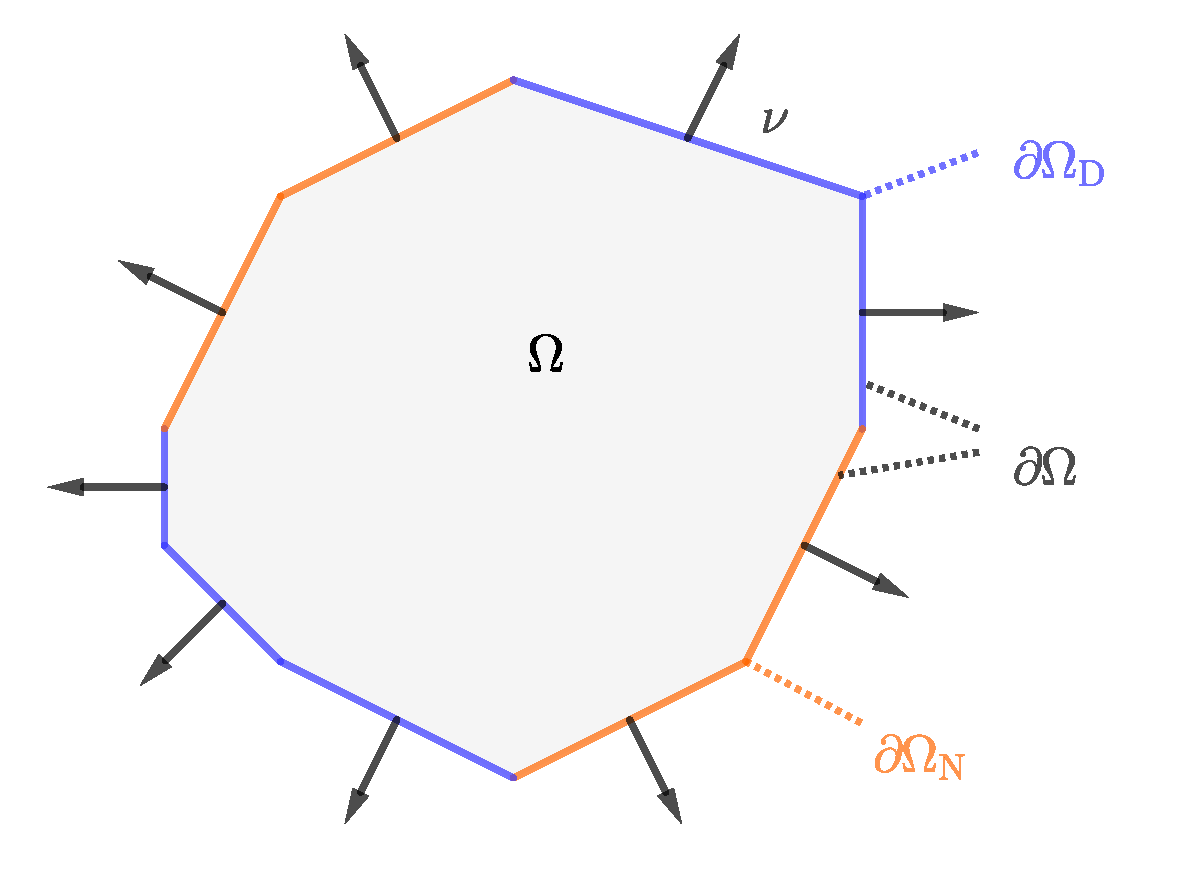
\includegraphics[width=0.5\textwidth]{images/domain.pdf}
          \caption[Beispiel eines zweidimensionalen Berechnungsgebietes]{%
            Die Abbildung zeigt ein schematisches Beispiel für ein zweidimensionales Berechnungsgebiet $\domain$.
            Der Rand $\boundary$ teilt sich dabei in $\dirichletBoundary$, auf dem Dirichlet-Randbedingungen herrschen, und $\neumannBoundary$, auf dem Neumann-Randbedingungen gelten sollen, ein.
            $ν$ beschreibt eine Funktion, die für fast-alle Punkte des Randes $\boundary$ deren äußere Normale angibt.
          }
          \label{fig:domain}
        \end{figure}
      % subsection berechnungsgebiet (end)

      \subsubsection{Poisson-Gleichung} % (fold)
      \label{ssub:poisson_gleichung}
        Die Poisson-Gleichung stellt eine wichtige Grundlage für die Wellen- und Wärmeleitungsgleichung dar.
        Sie ist eine zeitunabhängige, elliptische lineare partielle Differentialgleichung zweiter Ordnung und gerade aus diesem Grund als ein Test für die Implementierung geeignet.

        Gegeben seien zudem die folgenden Funktionen.
        \[
          f\in\setIntegrable^2(\domain)
          \separate
          u_\mathrm{D} \in \setSobolev^1(\domain)
          \separate
          u_\mathrm{N} \in \setIntegrable^2\roundBrackets{\neumannBoundary}
        \]
        Die Funktion $f$ ist auch bekannt als die Volumenkraft.
        Die Funktionen $u_\mathrm{D}$ und $u_\mathrm{N}$ stellen die Dirichlet- und Neumann-Randbedingungen dar.
        Gesucht ist nun eine Funktion $u\in\setSobolev^1(\domain)$, sodass die folgenden Gleichungen erfüllt sind.
        \begin{align*}
          -\laplacian u &= f \\
          u\vert_{\dirichletBoundary} &= u_\mathrm{D}\vert_{\dirichletBoundary} \\
          \scalarProduct{\nabla u\vert_{\neumannBoundary}}{ν} &= u_\mathrm{N}
        \end{align*}
        % Zu beachten ist, dass die Gleichungen im Sinne der punktweisen Gleichheit nur fast-überall erfüllt sein müssen.
        In diesem Falle stellt $u$ eine Lösung der Poisson-Gleichung dar.
        Nach dem Lemma von Lax und Milgram ist bekannt, dass für das gegebene Poisson-Problem eine schwache Lösung existiert.
        Aus diesem Grund bilden wir zunächst die schwache Formulierung des Poisson-Problems.
        Wir arbeiten die inhomogenen Dirichlet-Randbedingungen durch die folgende Zerlegung in das Problem ein.
        \[
          v\in\setSobolev^1_\mathrm{D}(\domain) \define \set{w\in\setSobolev^1(\domain)}{w\vert_{\dirichletBoundary} = 0}
        \]
        \[
          v\define u - u_\mathrm{D}
        \]
        Die schwache Formulierung ergibt sich dann zu der folgenden Form.
        Für alle $w\in\setSobolev^1_\mathrm{D}(\domain)$ muss das folgende gelten.
        \[
          \integral{\domain}{}{\scalarProduct{\nabla u}{\nabla w}}{λ} = \integral{\domain}{}{fw}{λ} + \integral{\neumannBoundary}{}{u_\mathrm{N}w}{σ} - \integral{\domain}{}{\scalarProduct{\nabla u_\mathrm{D}}{\nabla w}}{λ}
        \]
      % subsubsection poisson_gleichung (end)

      \subsubsection{Wärmeleitungsgleichung} % (fold)
      \label{ssub:wärmeleitungsgleichung}
        Die einfachste zeitabhängige PDE ist die Wärmeleitungsgleichung.

        \begin{align*}
          \partial_t u - \laplacian u &= f \\
          u(\cdot,t_0) &= u_0 \\
          u(\cdot,t)\vert_{\dirichletBoundary} &= u_\mathrm{D}\vert_{\dirichletBoundary} \\
          \scalarProduct{\nabla u(\cdot,t)\vert_{\neumannBoundary}}{ν} &= u_\mathrm{N}
        \end{align*}
      % subsubsection wärmeleitungsgleichung (end)

      \subsubsection{Wellengleichung} % (fold)
      \label{ssub:wellengleichung}
        \begin{align*}
          \partial^2_t u - \laplacian u &= f \\
          u(\cdot,t_0) &= u_0 \\
          \partial_t u(\cdot,t_0) &= u_1 \\
          u(\cdot,t)\vert_{\dirichletBoundary} &= u_\mathrm{D}\vert_{\dirichletBoundary} \\
          \scalarProduct{\nabla u(\cdot,t)\vert_{\neumannBoundary}}{ν} &= u_\mathrm{N}
        \end{align*}
      % subsubsection wellengleichung (end)

    % subsection modelprobleme (end)

    \subsection{Finite-Elemente-Methode} % (fold)
    \label{sub:finite_elemente_methode}
      Die Finite-Elemente-Methode ist, wie bereits in Abschnitt \ref{sec:introduction} erwähnt, ein allgemeines numerisches Verfahren, um partielle Differentialgleichungen approximativ zu lösen.
      Genauer gesagt, handelt es sich um eine spezielle Form des Ritz-Galerkin-Verfahrens.
      Die Finite-Elemente-Formulierung eines Problems resultiert in einem System von algebraischen Gleichungen.
      Um ein Problem zu lösen, unterteilt es das Berechnungsgebiet in kleinere und einfach zu behandelnde Teile (engl.: \textit{primitives}), die auch finite Elemente genannt werden.
      Die einfachen Systeme von algebraischen Gleichungen der einzelnen finiten Elemente werden dann in ein großes System von Gleichungen, welches das gesamte Problem modelliert, assembliert.
      Durch die Minimierung einer Fehlerfunktion mithilfe verschiedener Variationsmethoden ist die Finite-Elemente-Methode dann in der Lage, das Problem zu lösen.
      Im Folgenden wird die grundlegende Vorgehensweise an den Modelproblemen illustriert.

      \paragraph{Schritt 1: Konstruktion der schwachen Formulierung} % (fold)
      \label{par:schritt_1_konstruktion_der_schwachen_formulierung}
        \hfill\\
        Bereits in der Theorie ist es sinnvoll, die Lösungen von partiellen Differentialgleichungen in einer abgeschwächten Form zu verstehen, da bereits nicht stetige Quellterme die Forderungen an eine klassische Lösung verletzen \cite[S.~46]{Schweizer2013}.
        Demzufolge scheint eine klassische Formulierung von partiellen Differentialgleichungen für die numerische Mathematik ungeeignet.
        Für die Definition einer schwachen Lösung beziehungsweise schwachen Formulierung verallgemeinert man die Ableitung einer Funktion mithilfe von Distributionen \cite[S.~46~ff]{Schweizer2013}.
        In den Sobolevräumen werden dann die integrierbaren Funktionen zusammengefasst, die im Sinne einer Distribution wieder eine integrierbare Ableitung besitzen \cite[S.~54~ff]{Schweizer2013}.
      % paragraph schritt_1_konstruktion_der_schwachen_formulierung (end)

      \paragraph{Schritt 2: Diskretisierung des Berechnungsgebietes} % (fold)
      \label{par:schritt_2_diskretisierung_des_berechnungsgebietes}
        \hfill\\
        Aufgrund der Funktionsweise eines Computers ist man bei numerischen Simulationen gezwungen, kontinuierliche Probleme auf die eine oder andere Art und Weise zu diskretisieren.
        In der Finite-Elemente-Methode findet diese Diskretisierung durch die Einführung von finiten Elementen statt.
        Das Berechnungsgebiet $\domain$ und dessen Rand $\boundary$ werden in ein äquivalentes System von mehreren finiten Elementen überführt.
        Dabei wird die Anzahl, der Typ und die Größe dieser Elemente durch den Modellierer festgelegt.
        Für zwei Raumdimensionen werden zumeist Dreiecke und Vierecke gewählt.
        \begin{figure}[h]
          \center
          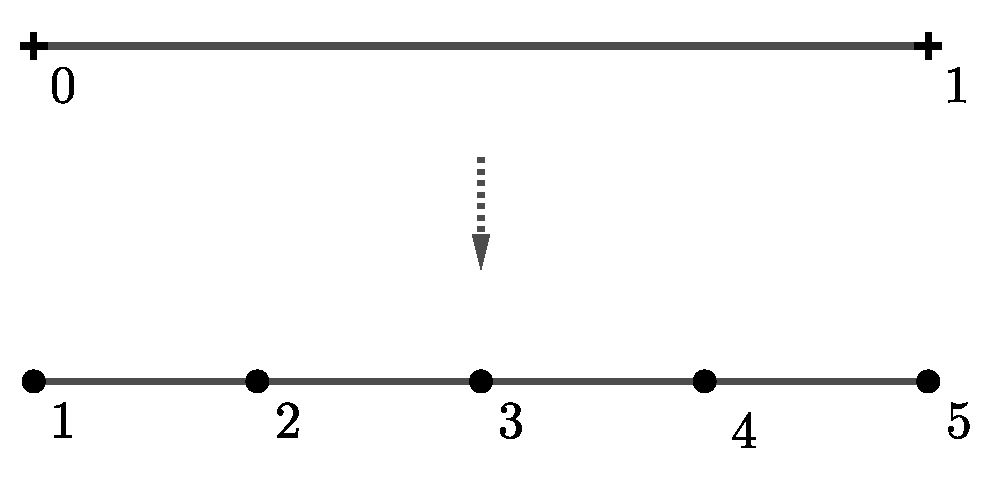
\includegraphics[width=0.5\textwidth]{images/domain_one_dimension_example.pdf}
          \caption[Diskretisierung eines eindimensionalen Berechnungsgebietes]{%
            Die Abbildung zeigt den Übergang von einem eindimensionalen Berechnungsgebiet in ein diskretisiertes Gebiet.
            Anstatt eines Intervalls wird das diskretisierte Gebiet nur noch durch Eckpunkte und deren Verbindungsstücke beschrieben.
          }
          \label{fig:domain-example}
        \end{figure}
        \begin{figure}[h]
          \begin{subfigure}[b]{0.5\textwidth}
            \center
            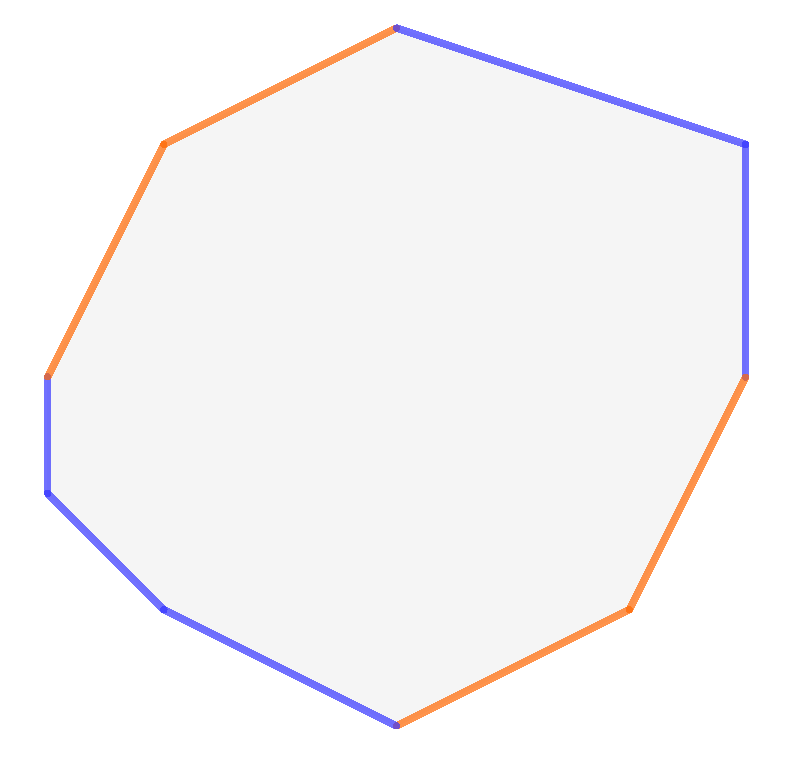
\includegraphics[width=0.6\textwidth]{images/domain_discretization_1.pdf}
          \end{subfigure}
          \begin{subfigure}[b]{0.5\textwidth}
            \center
            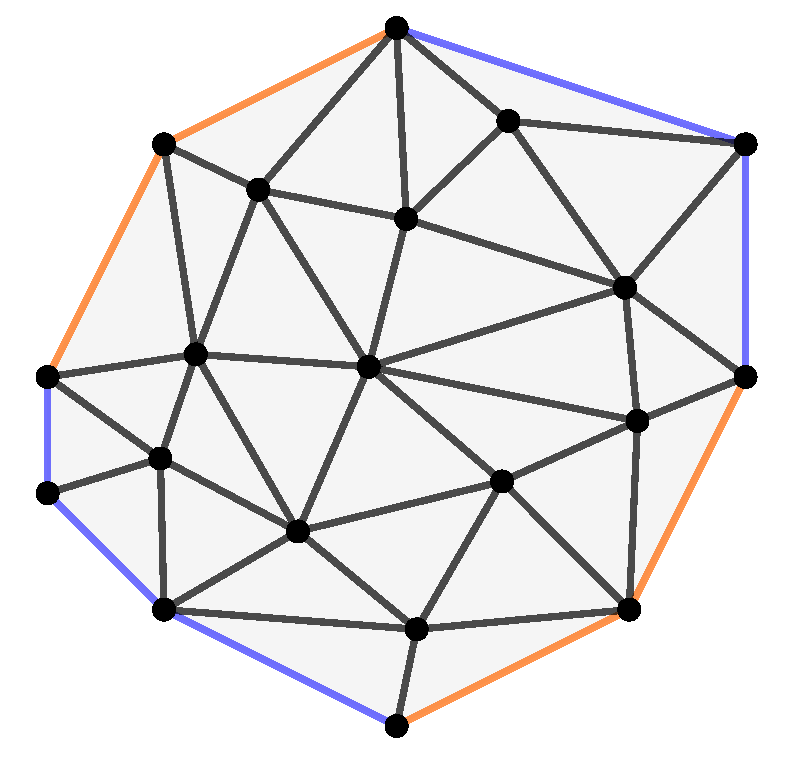
\includegraphics[width=0.6\textwidth]{images/domain_discretization_2.pdf}
          \end{subfigure}
          \caption[Diskretisierung eines zweidimensionalen Berechnungsgebietes]{%
            Die rechte Abbildung zeigt ein Beispiel für die Diskretisierung des polygonalen Berechnungsgebietes der linken Abbildung durch die Verwendung von Dreiecken.
            Die Dreiecke werden hierbei auch als finite Elemente bezeichnet.
          }
          \label{fig:domain-discretization}
        \end{figure}
      % paragraph schritt_2_diskretisierung_des_berechnungsgebietes (end)

      \paragraph{Schritt 3: Wahl der Basisfunktionen} % (fold)
      \label{par:schritt_3_wahl_der_basisfunktionen}
        \hfill\\
        Neben der Diskretisierung des Berechnungsgebietes $\domain$ ist auch die Diskretisierung der Funktionenräume $\setSobolev^1(\domain)$ und $\setSobolev^1_\mathrm{D}(\domain)$ nötig.
        Dies erreicht man durch die Wahl endlich vieler Basisfunktionen.
        Im Idealfall sollten diese einen kleinen Träger aufweisen, um die spätere Berechnung effizienter zu gestalten.
        Gerade für partielle Differentialgleichung zweiter Ordnung ist die Wahl von stückweise linearen Basisfunktionen ausreichend.
        \begin{figure}[h]
          \center
          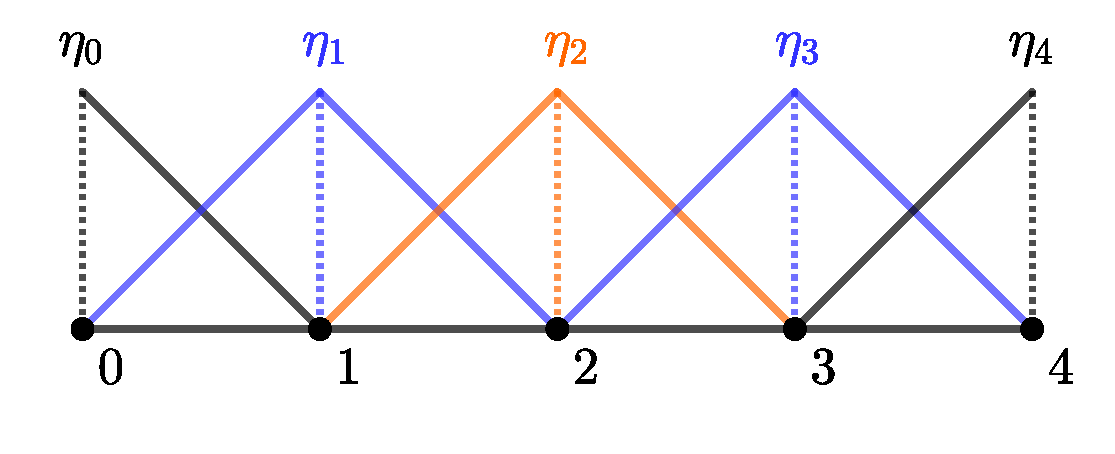
\includegraphics[width=0.5\textwidth]{images/hat_function_one_dimension_example.pdf}
          \caption[Eindimensionale Hutfunktionen]{%
            Die Abbildung zeigt die eindimensionalen Hutfunktionen $η_i$ für jeden Eckpunkt $i\in\set{0,1,2,3,4}{}$.
            Für den diskretisierten Raum von Funktionen stellen diese gerade die Basisfunktionen dar und beschreiben eine lineare Interpolation zwischen den Eckpunkten.
          }
          \label{fig:hat-function-example}
        \end{figure}
        \begin{figure}[h]
          \center
          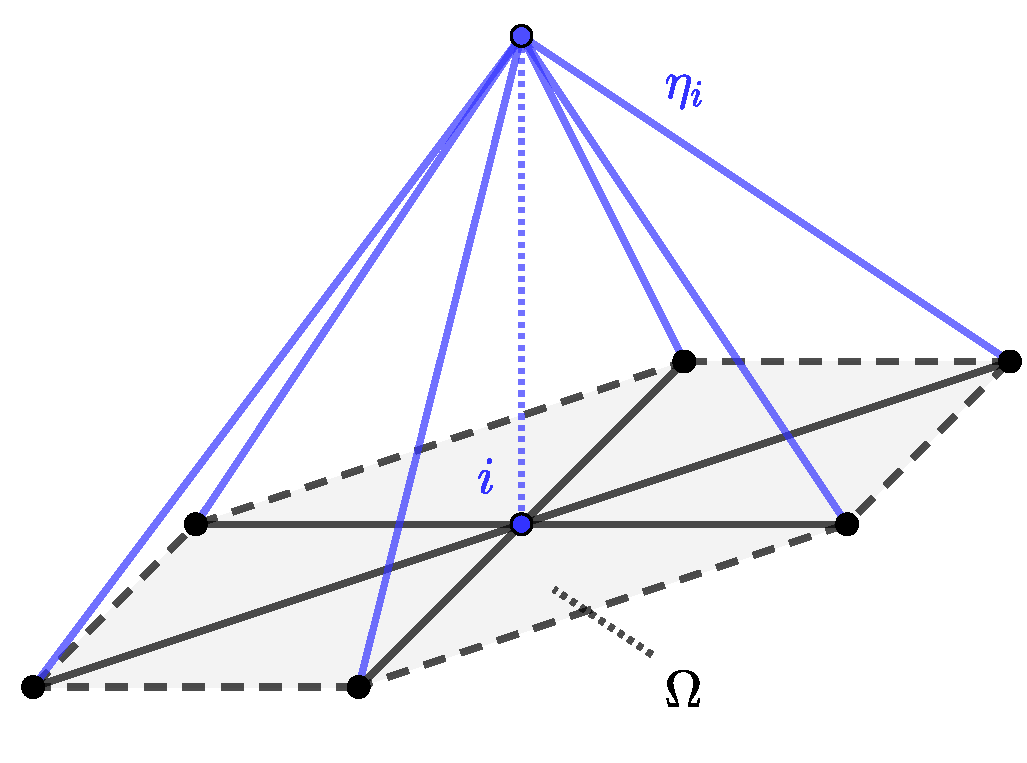
\includegraphics[width=0.5\textwidth]{images/hat_function.pdf}
          \caption[Zweidimensionale Hutfunktion]{%
            Die Abbildung zeigt die typische Wahl einer Basisfunktion $η_i$ über dem $i$.~Vertex des diskretisierten Berechnungsgebietes $\domain$.
            Aufgrund ihrer Form wird sie auch Hutfunktion genannt.
            Sie ist stückweise linear und identisch zu Null auf nicht benachbarten Dreiecken.
            Sie entspricht einer linearer Interpolation zwischen den Eckpunkten.
          }
          \label{fig:hat-function}
        \end{figure}
      % paragraph schritt_3_wahl_der_basisfunktionen (end)

      \paragraph{Schritt 4: Konstruktion der algebraischen Formulierung} % (fold)
      \label{par:schritt_4_konstruktion_der_algebraischen_formulierung}
        \hfill\\
        Das Einsetzen der Diskretisierung in die ursprüngliche schwache Formulierung der partiellen Differentialgleichung führt zu einem System von algebraischen Gleichungen.
        Die in dieser Arbeit besprochenen Fälle resultieren in linearen Gleichungssystemen mit dünnbesetzten Matrizen.
        Diese hängen zudem stark von der gewählten Diskretisierung ab.
        \[
          \roundBrackets{ \integral{\domain}{}{ \scalarProduct{\nabla η_i}{\nabla η_j} }{λ} }_{i,j} =
          \begin{pmatrix}
            1 & -1 & & & \\
            -1 & 2 & -1 & & \\
            & -1 & 2 & -1 & \\
            & & -1 & 2 & -1 \\
            & & & -1 & 1
          \end{pmatrix}
        \]
        \[
          \roundBrackets{ \integral{\domain}{}{ \scalarProduct{\nabla η_i}{\nabla η_j} }{λ} }_{i,j\in I} =
          \begin{pmatrix}
            2 & -1 & \\
            -1 & 2 & -1 \\
            & -1 & 2 \\
          \end{pmatrix}
        \]
      % paragraph schritt_4_konstruktion_der_algebraischen_formulierung (end)

      \paragraph{Schritt 5: Lösung des algebraischen Systems} % (fold)
      \label{par:schritt_5_lsen_des_algebraischen_systems}
        \hfill\\
        Die erhaltenen algebraischen Gleichungen sind äquivalent zu der schwachen Formulierung des diskretisierten Problems.
        In den hier betrachteten Fällen existieren eindeutige Lösungen.
      % paragraph schritt_5_lösen_des_algebraischen_systems (end)
    % subsection finite_elemente_methode (end)

    \subsection{Sparse Matrix Methoden} % (fold)
    \label{sub:sparse_matrix_methoden}

    % subsection sparse_matrix_methoden (end)

    \subsection{Aufbau und Funktionsweise des Grafikprozessors} % (fold)
    \label{sub:aufbau_und_funktionsweise_des_grafikprozessors}
      Der Grafikprozessor (GPU, engl.: \textit{graphics processing unit}) eines Computers stellt eine weitere Prozessorart gegenüber dem Hauptprozessor (CPU, engl: \textit{central processing unit}) dar.
      Im Gegensatz zur CPU ist der Aufbau und die Funktionsweise der GPU auf konkrete Aufgaben spezialisiert.
      In ihrer einfachsten Form generiert die GPU zwei- und dreidimensionale Grafiken, Bilder und Videos, die grafische Benutzeroberflächen, Computerspiele, Video- und Bildbearbeitung ermöglichen.
      Die moderne GPU ist ein massiv paralleler Multiprozessor optimiert für visuelle Berechnungen (engl.: \textit{visual computing}).
      Um dem Benutzer eine visuelle Interaktion in Echtzeit zu bieten, besitzt die GPU eine vereinheitlichte Grafik- und Prozessorarchitektur (engl.: \textit{graphics and computing architecture}).
      Diese dient sowohl als programmierbarer Grafikprozessor sowie als skalierbare parallele Plattform.
      Auf herkömmlichen Systemen werden zudem CPUs mit GPUs verbunden, um ein sogenanntes heterogenes System zu bilden, welches die Vorteile der jeweiligen Prozessorarten ausnutzt.
      \cite[S.~A3]{Patterson2011}

      Gerade bei parallelisierbaren Problemen mit kohärenten und linearen Speicherzugriffen, die auf Matrix- und Vektoroperationen aufbauen, stellt die Verwendung der GPU einen enormen Anstieg der Effizienz dar.
      Aus Abschnitt \ref{sub:finite_elemente_methode} wird ersichtlich, dass gerade ein Programm, welches auf der Finite-Elemente-Methode basiert, durch die GPU stark beschleunigt werden könnte.
      Auch die Auflösung der Diskretisierung des zugrundeliegenden Berechnungsgebietes könnte erhöht werden, da die GPU mit der Anzahl der finiten Elemente skalieren kann.

      \subsubsection{GPU Computing mit CUDA} % (fold)
      \label{ssub:gpu_computing_mit_cuda}
        \enquote{GPU Computing} ist das Ausnutzen der GPU für Berechnungen mithilfe einer parallelen Programmiersprache und einer Programmierschnittstelle (API, engl.: \textit{application programming interface}).
        Dies steht im Gegensatz zum ursprünglichen GPGPU-Modell (engl.: \textit{general purpose computation on GPU approach}), in welchem die GPU über traditionelle Graphik-APIs, wie zum Beispiel durch OpenGL GLSL, dazu gebracht wurde, Berechnungen durchzuführen, die nicht die Ausgabe eines Bildes auf dem Bildschirm zum Ziel hatten.
        Das von NVIDIA entwickelte CUDA ist ein skalierbares paralleles Programmiermodell, eine parallele Programmiersprache und  eine API, die es dem Programmierer erlauben, die typische Grafikschnittstelle der GPU zu umgehen und diese direkt durch die Sprachen C und C++ zu programmieren \cite[S.~A5]{Patterson2011}.
        Das CUDA-Programmiermodell arbeitet nach dem Prinzip \enquote{Single-Program Multiple Data} (SPMD).
        Der Programmierer schreibt hierbei ein Programm für einen einzelnen Thread, welches dann durch die GPU durch mehrere Threads instanziiert und ausgeführt wird \cite[S.~A5]{Patterson2011}.

        Für einen CUDA-Programmierer besteht ein Computersystem aus dem sogenannten \enquote{Host}, welcher in den meisten Fällen die CPU darstellt, und mindestens einer \enquote{Device}, die die GPU repräsentiert \cite[S.~39]{Kirk2010}.
        Ein CUDA-Programm teilt sich nun in mehrere Phasen, in denen Code entweder auf dem Host oder der Device ausgeführt wird, ein.
        Code der eine geringe Datenparallelität aufweist, wird dabei zumeist auf dem Host ausgeführt \cite{Kirk2010}.
        Umgekehrt sollte Code mit einer hohen Datenparallelität auf der GPU beziehungsweise der Device ausgeführt werden, um deren Vorteile zu nutzen \cite{Kirk2010}.
        Um bei der Ausführung des Quelltextes zwischen Host und Device wechseln zu können, bietet CUDA diverse Schnittstellen an.
        Ein CUDA-Programm startet zunächst auf dem Host, der durch den Aufruf eines entsprechenden \enquote{Kernels} in die Lage versetzt wird, Code auf mehreren Prozessoren der GPU auszuführen.
        Daten die zunächst nur im Arbeitsspeicher (RAM, engl.: \textit{random-access memory}) lagen und damit nur durch die CPU verwendbar waren, können durch CUDA bereit gestellte Befehle über den \enquote{PCI-Express Bus} (PCIe), der eine Datenverbindung zwischen der CPU und GPU bildet, in den dynamischen Arbeitsspeicher (DRAM, engl.: \textit{dynamic random-access memory}) der GPU übertragen werden.
        Zudem ist es dem Host auch möglich Daten vom DRAM der Device anzufordern.
        Auch diese werden dann über den PCIe in den RAM übertragen.
        \cite{Sanders2011}
      % subsubsection gpu_computing_mit_cuda (end)

      \subsubsection{Architektur einer modernen GPU} % (fold)
      \label{ssub:architektur_einer_modernen_gpu}
        Vereinheitlichte GPU-Architekturen basieren auf einer parallelen Anordnung von vielen programmierbaren Prozessoren, die auch die typischen Berechnungen für visuelle Ausgaben vollführen.
        Im Vergleich zu einer mehrkernigen CPU ist die Architektur einer GPU darauf ausgerichtet, extrem viele parallele Threads effizient auf einer großen Anzahl von Prozessorkernen auszuführen.
        In einer GPU wird diese Effizienz erreicht, indem man einfachere Prozessorkerne als in der CPU verwendet.
        Diese sind auf die Ausnutzung der Datenparallelität innerhalb einer Gruppe von Threads optimiert, sodass im Gegensatz zu einer CPU kleinere Caches und mehr Transistoren für arithmetische Einheiten verwendet werden können.
        \cite[S.~A11]{Patterson2011}

        \begin{figure}[h]
          \center
          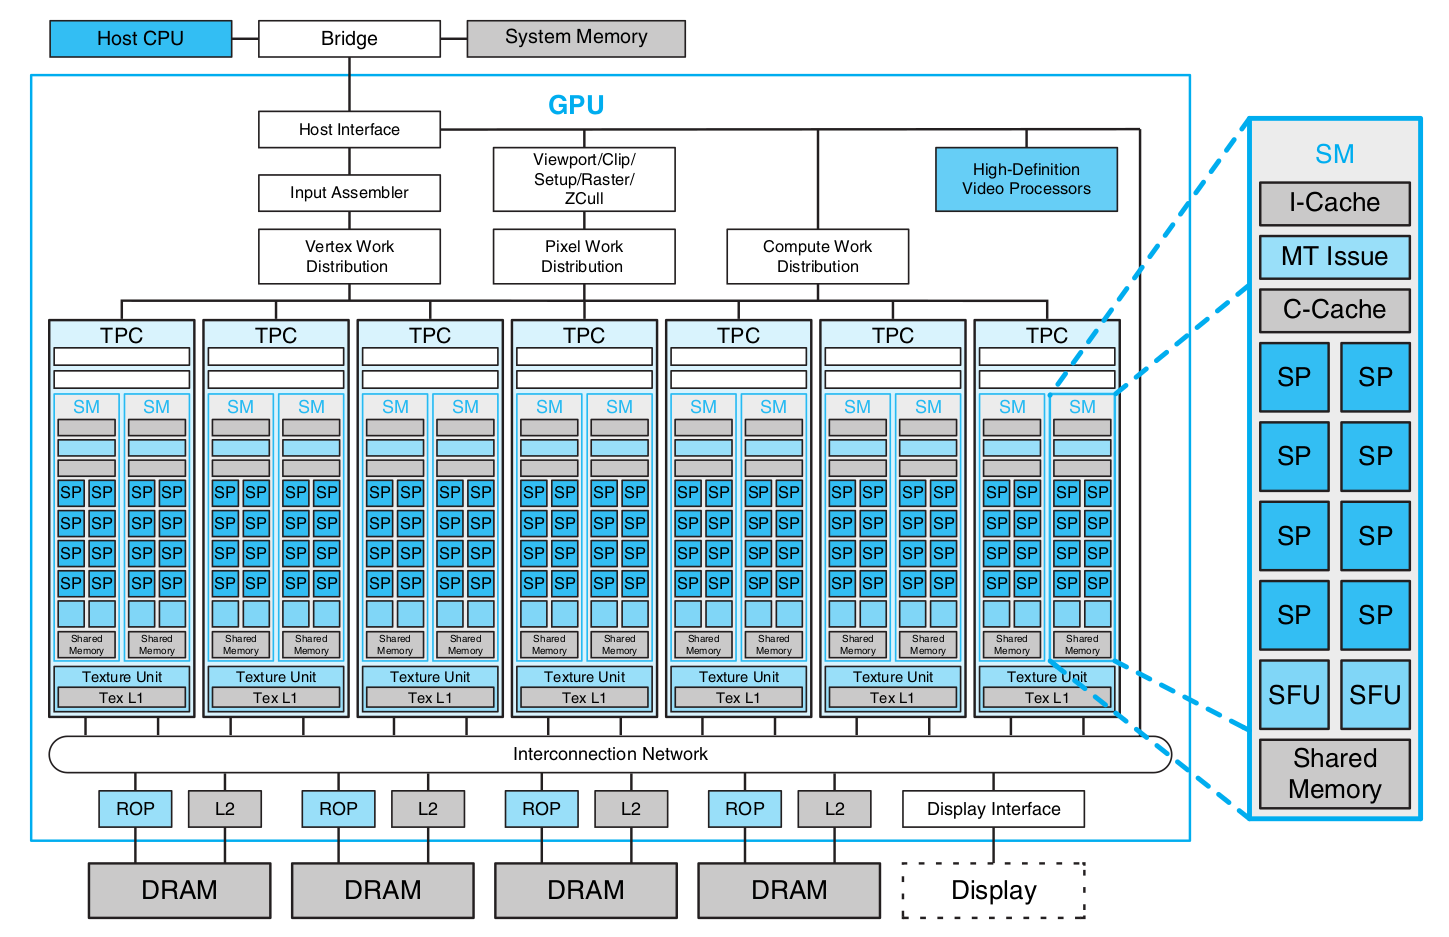
\includegraphics[width=0.95\textwidth]{images/unified_gpu_architecture.png}
          \caption[Grundlegende Architektur einer CUDA-fähigen GPU]{%
            Die Abbildung zeigt die grundlegende vereinheitlichte Architektur einer CUDA-fähigen GPU anhand eines Schemas.
            Es handelt sich dabei nur um Beispiele.
            \cite[S.~9]{Kirk2010}
          }
          \label{fig:gpu-architecture}
        \end{figure}

        Abbildung \ref{fig:gpu-architecture} skizziert die Architektur einer typischen CUDA-fähigen NVIDIA GPU.
        Sie besteht aus einem Feld von 112 \enquote{Streaming Processor Cores} (SP), die wiederum in 14 \enquote{Multithreaded Streaming Multiprocessors} (SM) eingeteilt sind.
        Jeder SP ist dazu in der Lage bis zu 100 parallele Threads in seiner Hardware zu organisieren und speichern.
        Die Prozessoren sind über ein Verbindungsnetzwerk mit Partitionen des dynamischen Arbeitsspeichers (DRAM, engl.: \textit{dynamic random-access memory}) verbunden.
        Zudem besitzt jeder SM \enquote{Special Function Units} (SFU), \enquote{Instruction Caches}, \enquote{Constant Caches}, \enquote{Multithreaded Instruction Units} und \enquote{Shared Memory}.
        Durch Hinzu- und Wegnahme von SMs und DRAM-Partitionen erhält man ein skalierbares Verfahren um schwächere und stärkere GPU-Konfigurationen zu konstruieren.
      % subsubsection architektur_einer_modernen_gpu (end)
    % subsection aufbau_und_funktionsweise_des_grafikprozessors (end)

  % section grundlagen (end)
\end{document}